\documentclass[landscape,a0paper,final,showframe]{baposter}

\usepackage{times}
\usepackage{calc}
\usepackage{graphicx}
\usepackage{amsmath}
\usepackage{amssymb}
\usepackage{relsize}
\usepackage{multirow}
\usepackage{bm}

\usepackage{graphicx}
\usepackage{multicol}

\usepackage{pgfbaselayers}
\pgfdeclarelayer{background}
\pgfdeclarelayer{foreground}
\pgfsetlayers{background,main,foreground}

\usepackage{helvet}
%\usepackage{bookman}
\usepackage{palatino}

\newcommand{\captionfont}{\footnotesize}

\selectcolormodel{cmyk}

\graphicspath{{images/}}

%%%%%%%%%%%%%%%%%%%%%%%%%%%%%%%%%%%%%%%%%%%%%%%%%%%%%%%%%%%%%%%%%%%%%%%%%%%%%%%%
%%%% Some math symbols used in the text
%%%%%%%%%%%%%%%%%%%%%%%%%%%%%%%%%%%%%%%%%%%%%%%%%%%%%%%%%%%%%%%%%%%%%%%%%%%%%%%%
% Format 
\newcommand{\Matrix}[1]{\begin{bmatrix} #1 \end{bmatrix}}
\newcommand{\Vector}[1]{\Matrix{#1}}
\newcommand*{\SET}[1]  {\ensuremath{\mathcal{#1}}}
\newcommand*{\MAT}[1]  {\ensuremath{\mathbf{#1}}}
\newcommand*{\VEC}[1]  {\ensuremath{\bm{#1}}}
\newcommand*{\CONST}[1]{\ensuremath{\mathit{#1}}}
\newcommand*{\norm}[1]{\mathopen\| #1 \mathclose\|}% use instead of $\|x\|$
\newcommand*{\abs}[1]{\mathopen| #1 \mathclose|}% use instead of $\|x\|$
\newcommand*{\absLR}[1]{\left| #1 \right|}% use instead of $\|x\|$

\def\norm#1{\mathopen\| #1 \mathclose\|}% use instead of $\|x\|$
\newcommand{\normLR}[1]{\left\| #1 \right\|}% use instead of $\|x\|$

%%%%%%%%%%%%%%%%%%%%%%%%%%%%%%%%%%%%%%%%%%%%%%%%%%%%%%%%%%%%%%%%%%%%%%%%%%%%%%%%
% Multicol Settings
%%%%%%%%%%%%%%%%%%%%%%%%%%%%%%%%%%%%%%%%%%%%%%%%%%%%%%%%%%%%%%%%%%%%%%%%%%%%%%%%
\setlength{\columnsep}{0.7em}
\setlength{\columnseprule}{0mm}


%%%%%%%%%%%%%%%%%%%%%%%%%%%%%%%%%%%%%%%%%%%%%%%%%%%%%%%%%%%%%%%%%%%%%%%%%%%%%%%%
% Save space in lists. Use this after the opening of the list
%%%%%%%%%%%%%%%%%%%%%%%%%%%%%%%%%%%%%%%%%%%%%%%%%%%%%%%%%%%%%%%%%%%%%%%%%%%%%%%%
\newcommand{\compresslist}{%
\setlength{\itemsep}{1pt}%
\setlength{\parskip}{0pt}%
\setlength{\parsep}{0pt}%
}


%%%%%%%%%%%%%%%%%%%%%%%%%%%%%%%%%%%%%%%%%%%%%%%%%%%%%%%%%%%%%%%%%%%%%%%%%%%%%%
%%% Begin of Document
%%%%%%%%%%%%%%%%%%%%%%%%%%%%%%%%%%%%%%%%%%%%%%%%%%%%%%%%%%%%%%%%%%%%%%%%%%%%%%

\begin{document}

%%%%%%%%%%%%%%%%%%%%%%%%%%%%%%%%%%%%%%%%%%%%%%%%%%%%%%%%%%%%%%%%%%%%%%%%%%%%%%
%%% Here starts the poster
%%%---------------------------------------------------------------------------
%%% Format it to your taste with the options
%%%%%%%%%%%%%%%%%%%%%%%%%%%%%%%%%%%%%%%%%%%%%%%%%%%%%%%%%%%%%%%%%%%%%%%%%%%%%%
\typeout{Poster Starts}
%\background{
 % \begin{tikzpicture}[remember picture,overlay]%
  %  \draw (current page.north west)+(-2em,-0em) node[anchor=north west] {\hspace{-2em}\includegraphics[height=1.1\textheight]{silhouettes_background}};
 % \end{tikzpicture}%
%}
\definecolor{silver}{cmyk}{0,0,0,0.3}
\definecolor{yellow}{cmyk}{0,0,0.9,0.0}
\definecolor{reddishyellow}{cmyk}{0,0.22,1.0,0.0}
\definecolor{black}{cmyk}{0,0,0.0,1.0}
\definecolor{darkYellow}{cmyk}{0,0,1.0,0.5}
\definecolor{darkSilver}{cmyk}{0,0,0,0.1}

\definecolor{uclagold}{cmyk}{0,.29,.91,0}
\definecolor{uclablue}{cmyk}{.75,.35,0,.07}
\definecolor{lightyellow}{cmyk}{0,0,0.3,0.0}
\definecolor{lighteryellow}{cmyk}{0,0,0.1,0.0}
\definecolor{lightestyellow}{cmyk}{0,0,0.05,0.0}
\begin{poster}{
  % Show grid to help with alignment
  grid=no,
  % Column spacing
  colspacing=1em,
  % Color style
  bgColorOne=white,
  bgColorTwo=white,
  %borderColor=uclablue,
  borderColor=uclagold,
  headerColorOne=white,
  %headerColorTwo=yellow,
  headerColorTwo=uclagold,
  headerFontColor=black,
  %boxColorOne=lightyellow,
  %boxColorTwo=lighteryellow,
  % Format of textbox
  textborder=faded,
  % Format of text header
  eyecatcher=no,
  headerborder=open,
  headerheight=0.09\textheight,
  headershape=roundedright,
  headershade=shade-lr,
  headerfont=\Large\textsf, %Sans Serif
  boxshade=shade-lr,
  background=shade-tb,
  %background=none,
  linewidth=2pt
  }
  % Eye Catcher
  {} % No eye catcher for this poster. If an eye catcher is present, the title is centered between eye-catcher and logo.
  % Title
  {\textnormal{\sf%Sans Serif
  % Serif
 Earthquake forecast evaluation using space-time point process residual analysis}}
  % Authors
  {\sf %Sans Serif
  % Serif
  Robert Alan Clements$^1$, Frederic Paik Schoenberg$^1$, and Danijel Schorlemmer$^2$\hspace{3em} \\
  {\footnotesize $^1$UCLA Department of Statistics, $^2$USC Southern California Earthquake Center}
 % brian.amberg@unibas.ch\hspace{3em}
  %University of Basel, Switzerland
  }
   % University logo
  {{\begin{minipage}{5em}
    \hfill
    \includegraphics[height=4em]{ucla}
   % \includegraphics[height=5.5em]{logo}
  \end{minipage}}
  }

  \tikzstyle{light shaded}=[top color=baposterBGtwo!30!white,bottom color=baposterBGone!30!white,shading=axis,shading angle=30]

  % Width of left inset image
     \newlength{\leftimgwidth}
     \setlength{\leftimgwidth}{0.78em+8.0em}

%%%%%%%%%%%%%%%%%%%%%%%%%%%%%%%%%%%%%%%%%%%%%%%%%%%%%%%%%%%%%%%%%%%%%%%%%%%%%%
%%% Now define the boxes that make up the poster
%%%---------------------------------------------------------------------------
%%% Each box has a name and can be placed absolutely or relatively.
%%% The only inconvenience is that you can only specify a relative position 
%%% towards an already declared box. So if you have a box attached to the 
%%% bottom, one to the top and a third one which should be in between, you 
%%% have to specify the top and bottom boxes before you specify the middle 
%%% box.
%%%%%%%%%%%%%%%%%%%%%%%%%%%%%%%%%%%%%%%%%%%%%%%%%%%%%%%%%%%%%%%%%%%%%%%%%%%%%%
    %
    % A coloured circle useful as a bullet with an adjustably strong filling
    \newcommand{\colouredcircle}[1]{%
      \tikz{\useasboundingbox (-0.2em,-0.32em) rectangle(0.2em,0.32em); \draw[draw=black,fill=baposterBGone!80!black!#1!white,line width=0.03em] (0,0) circle(0.18em);}}

%%%%%%%%%%%%%%%%%%%%%%%%%%%%%%%%%%%%%%%%%%%%%%%%%%%%%%%%%%%%%%%%%%%%%%%%%%%%%%
  \headerbox{Introduction}{name=contribution,column=0,row=0}{
%%%%%%%%%%%%%%%%%%%%%%%%%%%%%%%%%%%%%%%%%%%%%%%%%%%%%%%%%%%%%%%%%%%%%%%%%%%%%%
   {}A collection of earthquake (eq) forecast models from the Collaboratory for the Study of EQ Predictability have traditionally been tested using numerical summaries and error diagrams. Here, we propose using residual analysis methods for space-time point processes to evaluate and compare a subset of these models. Residuals such as these can help reveal specific locations where the forecast is failing.
 }

%%%%%%%%%%%%%%%%%%%%%%%%%%%%%%%%%%%%%%%%%%%%%%%%%%%%%%%%%%%%%%%%%%%%%%%%%%%%%%
  \headerbox{EQ Forecast Models}{name=model,column=0,below=contribution}{
%%%%%%%%%%%%%%%%%%%%%%%%%%%%%%%%%%%%%%%%%%%%%%%%%%%%%%%%%%%%%%%%%%%%%%%%%%%%%%
Each model forecasts a rate of eqs in space-time-magnitude bins in California. Models are divided into 1-day models (ETAS and STEP) and 5-year models (A1 [3], B1 [4], and C1 [5]) with forecast period 2006-2011. 1-day models forecast eqs of M $\geq$ 3.95. 5-year models are extrapolated to forecast eqs of M $\geq$ 3.95. 
\vspace{.9em}\\
\begin{tabular}{cc}
	ETAS & \hspace{2.5em}STEP \\
	\includegraphics[height=.42\linewidth]{etas.png} & \hspace{2.5em}\includegraphics[height=.42\linewidth]{step.png} \\
%\end{tabular}
%\begin{tabular}{cc}
	A1 & \hspace{2.5em}B1 \\
	\includegraphics[height=.42\linewidth]{helm.png} & \hspace{2.5em}\includegraphics[height=.42\linewidth]{kagan.png} \\
%\end{tabular}
%\begin{tabular}{cc}
\end{tabular}
\begin{center}
	C1  \\
	\includegraphics[height=.42\linewidth]{shen.png}  %& \hspace{2.5em}\includegraphics[height=.45\linewidth]{helmeqs.pdf}
%\end{tabular}
\end{center}
  }

\headerbox{Conditional Intensity}{name=pp, column=1, row=0}{
EQ occurrences can be modeled as a space-time point process, $N$, defined on a compact set, $\mathcal{S} \subset \mathbb{R}^{d}$. To model $N$, one typically models the conditional intensity $\lambda(\mathbf{x}|\mathcal{H}_{t}) < \infty$, defined as the rate at which eqs are expected to occur around a location $\mathbf{x}$, given the prior history $\mathcal{H}_{t}$. 
}
%%%%%%%%%%%%%%%%%%%%%%%%%%%%%%%%%%%%%%%%%%%%%%%%%%%%%%%%%%%%%%%%%%%%%%%%%%%%%%
  \headerbox{Pixel-based Residuals}{name=fitting,column=1,below=pp}{
%%%%%%%%%%%%%%%%%%%%%%%%%%%%%%%%%%%%%%%%%%%%%%%%%%%%%%%%%%%%%%%%%%%%%%%%%%%%%%
The testing region, $\mathcal{S}$, is divided into bins, $B_{i}$. Residuals can then be computed within each $B_{i}$ using the estimated model for the conditional intensity, $\hat{\lambda}$.\\
%\vspace{.1cm} 
% \textit{ \textbf{Raw residuals}} [4]: \\
%  \vspace{.1em}\\
%$R_{R}(B_{i}) = N(B_{i}) - \int_{{B_{i}}}\hat{\lambda}(\mathbf{x}|{\mathcal{H}_{t}}) d\mathbf{x}$ \\
%\vspace{.1em}\\
\textit{\textbf{Pearson residuals}} [1]: \\
\vspace{.1em}\\
$R_{P}(B_{i}) = \sum_{(\mathbf{x}_{i}) \in B_{i}}\frac{1}{\sqrt{\hat{\lambda}(\mathbf{x}_{i}|\mathcal{H}_{t})}} - \int_{B_{i}}\sqrt{\hat{\lambda}(\mathbf{x}|\mathcal{H}_{t})}d\mathbf{x}$ \\
\vspace{.1em}\\
\textit{\textbf{Deviance residuals}} of Model 1 vs Model 2 [5] (a model comparison tool):
\begin{align*}
R_{D}(B_{i}) &= \sum_{(\mathbf{x}_{i}) \in B_{i}} \log{\hat{\lambda}_{1}} - \int_{B_{i}}\hat{\lambda}_{1}d\mathbf{x} \\
 &- \left( \sum_{(\mathbf{x}_{i}) \in B_{i}} \log{\hat{\lambda}_{2}} - \int_{B_{i}}\hat{\lambda}_{2}d\mathbf{x}\right)
 \end{align*}
}

%%%%%%%%%%%%%%%%%%%%%%%%%%%%%%%%%%%%%%%%%%%%%%%%%%%%%%%%%%%%%%%%%%%%%%%%%%%%%%


%%%%%%%%%%%%%%%%%%%%%%%%%%%%%%%%%%%%%%%%%%%%%%%%%%%%%%%%%%%%%%%%%%%%%%%%%%%%%%
  \headerbox{Super-thinned residuals}{name=tresids,column=1,below=fitting}{
%%%%%%%%%%%%%%%%%%%%%%%%%%%%%%%%%%%%%%%%%%%%%%%%%%%%%%%%%%%%%%%%%%%%%%%%%%%%%%
 % \begin{tabular}{@{}c@{ }c@{ }c@{ }c@{}@{ }@{ }c@{ }c@{ }c@{ }c@{ }}
  %  \includegraphics[height=0.42\linewidth]{16_1_tgt}&
  %  \includegraphics[height=0.42\linewidth]{16_1_expression}&
  %  \includegraphics[height=0.42\linewidth]{16_1_neutral}\\[-0.8em]
 %   \smaller a) Target & \smaller b) Fit & \smaller c) Normalized\\[0.8em]
  %  \includegraphics[height=0.42\linewidth]{16_6_tgt}&
  %  \includegraphics[height=0.42\linewidth]{16_6_expression}&
  %  \includegraphics[height=0.42\linewidth]{16_6_neutral}\\[-0.8em]
  %  \smaller a) Target & \smaller b) Fit & \smaller c) Normalized
 % \end{tabular}
Using the super-thinning method, $N$ can be transformed into $Z$, a homogeneous Poisson process, iff $\hat{\lambda} = \lambda$. Any clustering, inhibition, or spatial trend in $Z$ is indicative of a lack-of-fit in those locations. 
 \vspace{-.5em}
 \begin{itemize}
	\item \textbf{superpose} points if $\hat{\lambda}(\mathbf{x}|\mathcal{H}_{t}) < k$,\\ inf$\{\hat{\lambda}\} \leq k \leq $ sup$\{\hat{\lambda}\}$
		\vskip.1em
		\begin{itemize}
			\item simulate points with rate $k - \hat{\lambda}(\mathbf{x}|\mathcal{H}_{t})$
		\end{itemize}
		\vskip.1em
		\item \textbf{thin} points if $\hat{\lambda}(\mathbf{x}_{i}|\mathcal{H}_{t}) \geq k$
		\vskip.1em
		\begin{itemize}
			\item keep each point with probability ${k}/{\hat{\lambda}(\mathbf{x}_{i}|\mathcal{H}_{t})}$
		\end{itemize}
		\vskip.1em
		\item the result, called \textbf{\textit{super-thinned}} residuals, is homogeneous Poisson, with rate $k$, iff $\hat{\lambda} = \lambda$ [2]
	\end{itemize}
  }
%%%%%%%%%%%%%%%%%%%%%%%%%%%%%%%%%%%%%%%%%%%%%%%%%%%%%%%%%%%%%%%%%%%%%%%%%%%%%%
%%%%%%%%%%%%%%%%%%%%%%%%%%%%%%%%%%%%%%%%%%%%%%%%%%%%%%%%%%%%%%%%%%%%%%%%%%%%%%
  \headerbox{Results}{name=results,column=2,span=2,row=0}{
%%%%%%%%%%%%%%%%%%%%%%%%%%%%%%%%%%%%%%%%%%%%%%%%%%%%%%%%%%%%%%%%%%%%%%%%%%%%%%
 \mbox{\hspace{2cm}} {\large Pearson residuals}\hspace{4cm} {\large Super-thinned residuals}\\
 %
\vspace{-.3cm}\\
%
 \mbox{\hspace{3.3cm}} B1 \hspace{5.6cm} (a) A1 \hspace{.9cm}(b) B1 \hspace{.9cm}(c) C1 \\
 \vspace{-.8cm}\\
\begin{tabular}{cc}
	\hspace{1.2cm}  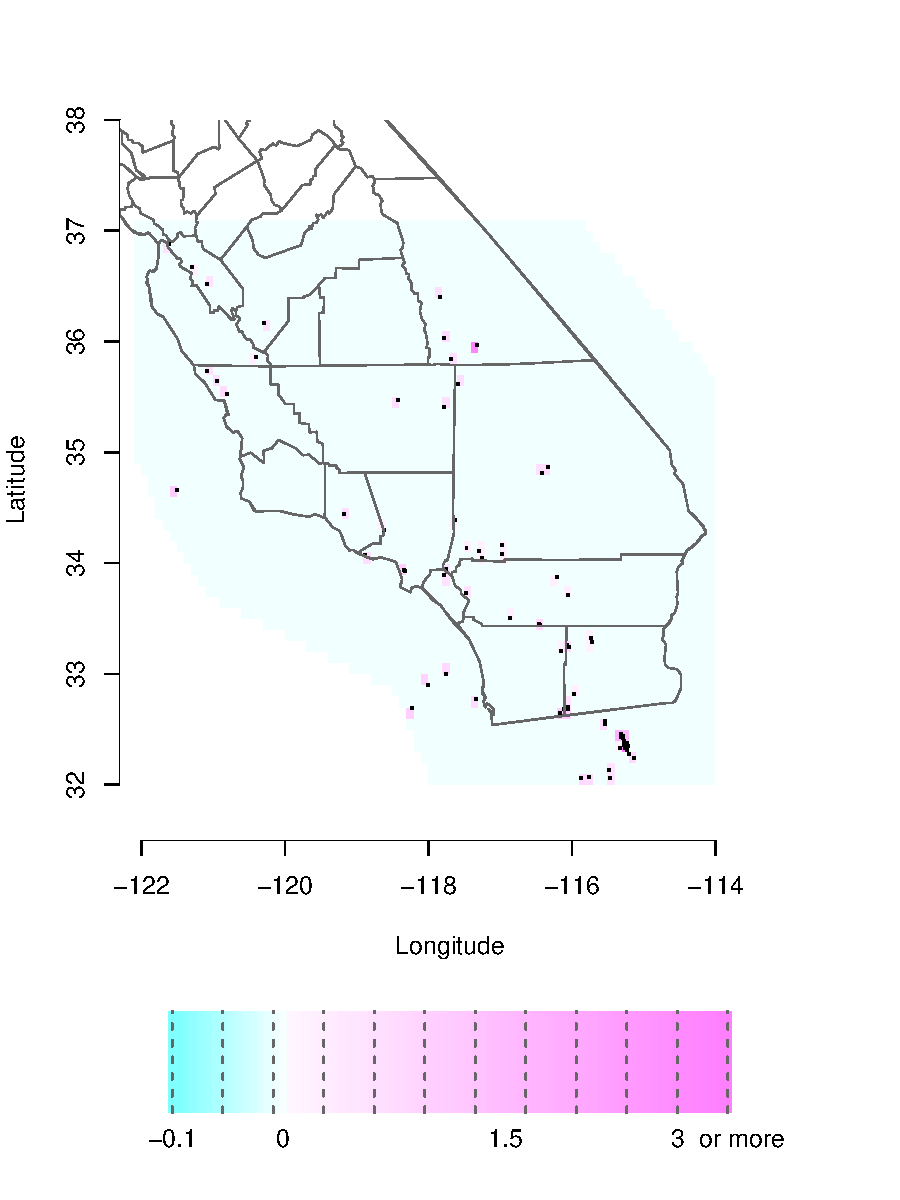
\includegraphics[height=.4\linewidth]{kaganxtPearsonnew.pdf}  & \hspace{2cm}
	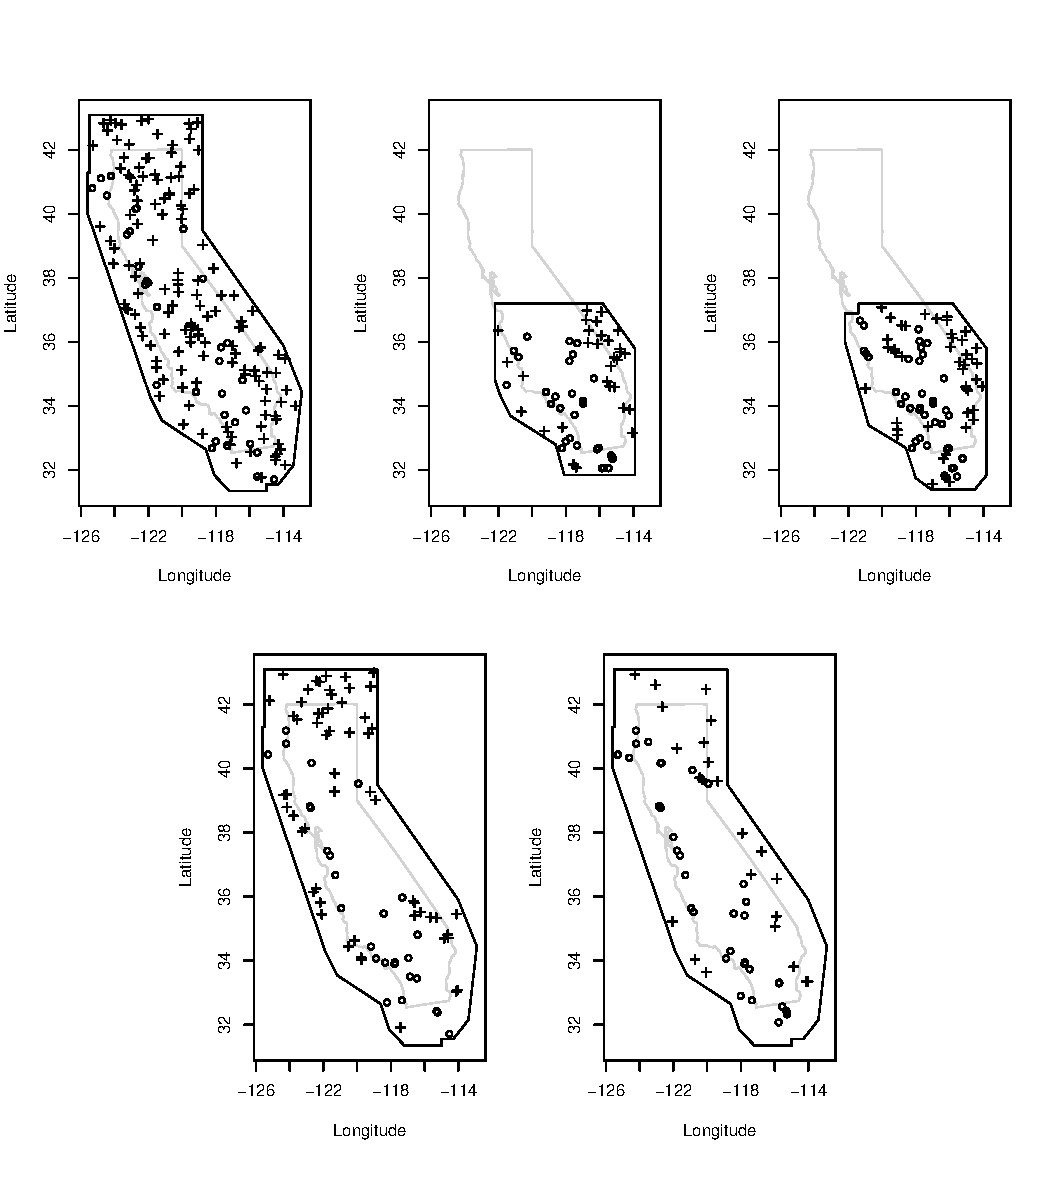
\includegraphics[height=.4\linewidth]{allst.pdf}
\end{tabular}
\vspace{-.4cm}\\
\mbox{\hspace{10.2cm}} (d) ETAS \hspace{.4cm} (e) STEP\\
\vspace{-.3cm}\\
The Pearson residuals typically reveal only the largest residuals which tend to occur in bins containing eqs. Clustering leftover in the Imperial fault zone (directly south of the California-Mexico border), and large areas of empty space in the super-thinned residuals imply under-prediction and over-prediction, respectively.  
%
\vspace{-.1cm}\\
 \mbox{\hspace{0.1\linewidth}\rule{0.8\linewidth}{1pt}\hspace{0.1\linewidth}}\\
 %
 \vspace{-.7cm}
\begin{center}\large{{Deviance residuals}} \end{center}
%
\vspace{-.3cm}
%
\begin{tabular}{ccc}
\hspace{.1\linewidth}{(a) A1 vs B1} & \hspace{.18\linewidth}{(b) A1 vs C1} & \hspace{.2\linewidth}{(c) B1 vs C1} 
\end{tabular}\\ \vspace{-1cm}\\
\begin{tabular}{ccc}
	\includegraphics[height=.42\linewidth]{helmxtvkaganxtdevnew3.pdf} & \includegraphics[height=.42\linewidth]{helmxtvshenxtdevnew3.pdf} & \includegraphics[height=.42\linewidth]{kaganxtvshenxtdevnew5.pdf}
\end{tabular}
pink $\implies$ Model 1 is preferred; blue $\implies $ Model 2 is preferred. Overall, Model A1 > C1 > B1; ETAS > STEP (not shown). The results indicate over-prediction of seismicity in inter-fault zones for A1; under-prediction in B1 and C1 around the Imperial, Laguna Salada, Baja, and Panamint clusters.
 %
%\vspace{-.2cm}
%\hspace{.1cm} \large{{Super-thinned residuals}} \hspace{.1cm} \large{{Pearson residuals for B1}}
       %   \mbox{\hspace{0.3\linewidth}\rule{0.4\linewidth}{1pt}\hspace{0.3\linewidth}}\\
   %   \begin{tabular}{cc}
    %    \hspace{0.5em}\scalebox{0.74}{\input{shrec_MNCG}} &
    %    \hspace{0.5em}\scalebox{0.74}{\input{und_MNCG}}
   %   \end{tabular}\\
%      \begin{multicols}{2}
      %      \end{multicols}\vspace{-1em}
    %  \begin{tabular}{cc}
     %   \hspace{0.5em}\scalebox{0.74}{\input{shrec_PR}} &
     %   \hspace{0.5em}\scalebox{0.74}{\input{und_PR}}
   %   \end{tabular}\\
%      \begin{multicols}{2}
%      \end{multicols}\vspace{-1em}
   %   \begin{tabular}{cc}
    %    \hspace{0.5em}\scalebox{0.74}{\input{shrec_FARFRR}} &
    %    \hspace{0.5em}\scalebox{0.74}{\input{und_FARFRR}}
   %   \end{tabular}\\
%      \begin{multicols}{2}
%      \end{multicols}
  }%
%%%%%%%%%%%%%%%%%%%%%%%%%%%%%%%%%%%%%%%%%%%%%%%%%%%%%%%%%%%%%%%%%%%%%%%%%%%%%%
%%%%%%%%%%%%%%%%%%%%%%%%%%%%%%%%%%%%%%%%%%%%%%%%%%%%%%%%%%%%%%%%%%%%%%%%%%%%%%
%%%%%%%%%%%%%%%%%%%%%%%%%%%%%%%%%%%%%%%%%%%%%%%%%%%%%%%%%%%%%%%%%%%%%%%%%%%%%%
  \headerbox{References}{name=references,column=2, span=2, above=bottom,below=results}{
%%%%%%%%%%%%%%%%%%%%%%%%%%%%%%%%%%%%%%%%%%%%%%%%%%%%%%%%%%%%%%%%%%%%%%%%%%%%%%
    \tiny
    \vspace{-0.4em}
    \bibliographystyle{ieee}
    \renewcommand{\section}[2]{\vskip 0.05em}
      \begin{thebibliography}{1}\itemsep=-.8em
      \setlength{\baselineskip}{0.4em}
      \bibitem{amberg07:nonrigid}
        A.~Baddeley, R.~Turner, J.~Moller, and M.~Hazelton (2005).
        \newblock {R}esidual analysis for spatial point processes. 
        \newblock {\em JRSS} \textbf{67} 617-666. 
      \bibitem{amberg08:recognition}
        R.~Clements, F.~Schoenberg, and A.~Veen (2010).
        \newblock Evaluation of space-time point process models using super-thinning.
        \newblock {\em UCLA Statistics Preprints} \textbf{579}.
          \bibitem{amberg08:recognition}
        A.~Helmstetter, Y.~Kagan, and D.~Jackson (2007).
        \newblock High-resolution time-independent grid-based forecast M$\geq$5 earthquakes in California.
        \newblock {\em SRL} \textbf{78} 78-86.
          \bibitem{amberg08:recognition}
        Y.~Kagan, D.~Jackson, and Y.~Rong (2007).
        \newblock A testable five-year forecast of moderate and large earthquakes in southern California based on smoothed seismicity.
        \newblock {\em SRL} \textbf{78} 94-98.
          \bibitem{amberg08:recognition}
        Z.~Shen, D.~Jackson, and Y.~Kagan (2007).
        \newblock Implications of geodetic strain rate for future earthquakes, with a five-year forecast of M5 earthquakes in southern California.
        \newblock {\em SRL} \textbf{78} 116-120.
        \bibitem{amberg08:recognition}
        K.~Wong and F.~Schoenberg (2010).
        \newblock On mainshock focal mechanisms and the spatial distribution of aftershocks.
        \newblock {\em In review}.
      \end{thebibliography}
  }%
\end{poster}%
%
\end{document}
